\documentclass[aspectratio=169,10pt]{beamer}

\usetheme{metropolis}
\usepackage{booktabs}
\usepackage{array}
\usepackage{graphicx}
\usepackage{xcolor}
\usepackage{tikz}
\usetikzlibrary{positioning,arrows.meta,shapes.geometric,fit,backgrounds}
\usepackage{amsmath}
\usepackage{colortbl}

\tikzset{
  block/.style={rectangle, draw=brand!70, fill=brand!10, rounded corners=2pt,
                minimum height=5mm, minimum width=14mm, font=\scriptsize, inner sep=2pt, align=center},
  op/.style={rectangle, draw=accent!70, fill=accent!10, rounded corners=2pt,
             minimum height=5mm, minimum width=14mm, font=\scriptsize, inner sep=2pt, align=center},
  label/.style={font=\tiny, text=neutral},
  arr/.style={-{Stealth[length=1.4mm]}, thick, draw=neutral},
}

\definecolor{brand}{HTML}{1F4E79}
\definecolor{accent}{HTML}{C0504D}
\definecolor{good}{HTML}{2E7D32}
\definecolor{neutral}{HTML}{555555}
\setbeamercolor{frametitle}{bg=brand,fg=white}
\setbeamercolor{progress bar}{fg=accent}

\title{Extracting Social and Clinical Impacts of Substance Use from Reddit}
\subtitle{CE7455 Project -- Group G26}
\author{Ismail Elyamany \and Huang Chongtian \and Xia Yitong \and Zhu Ruijie}
\institute{Nanyang Technological University}
\date{April 2026}

\newcommand{\sota}{\textcolor{accent}{\textbf{0.610}}}
\newcommand{\ours}{\textcolor{good}{\textbf{0.635}}}
\newcommand{\bestsingle}{\textcolor{good}{\textbf{0.613}}}

\begin{document}

% ---------- 1. Title ----------
\begin{frame}[plain]
  \titlepage
\end{frame}

% ---------- 2. The Task ----------
\begin{frame}{The Task: Impact Extraction from Reddit}
  \textbf{SMM4H--HeaRD 2026 Task 7 Contest } Token-level NER on opioid-subreddit posts.
  \medskip

  Task: To identify two entity types using BIO tagging:
  \begin{itemize}
    \item \textcolor{brand}{\textbf{ClinicalImpacts}} -- for e.g. overdose, withdrawal, depression, insomnia \ldots
    \item \textcolor{accent}{\textbf{SocialImpacts}} -- for e.g. job loss, arrest, homelessness, broken relationships \ldots
  \end{itemize}

  \medskip
  \textbf{Example}
  \begin{quote}\small
    ``I lost \textcolor{accent}{\underline{my job}} last month and ever since I've had
    \textcolor{brand}{\underline{constant panic attacks}}.''
  \end{quote}

  \vfill
  \textbf{Motivation} \\Useful for population-level signal mining from user-generated text -- public health surveillance, harm-reduction research.
\end{frame}

% ---------- 3. Why It's Hard ----------
\begin{frame}{Why It's Hard}
  \begin{columns}[T,onlytextwidth]
    \column{0.55\textwidth}
      \textbf{1. Train/Test Distribution Shift}
      \begin{itemize}
        \item Train is 75\% Clinical, 25\% Social.
        \item Test is $\approx$30\% Clinical, 70\% Social.
        \item Models trained on Train over-predict Clinical.
      \end{itemize}
      \medskip

      \textbf{2. Implicit, Colloquial Language}
      \begin{itemize}
        \item ``those weeks were hell'' (Clinical)
        \item ``I lost everything'' (Social)
        \item No clinical vocabulary, no named triggers.
      \end{itemize}
    \column{0.45\textwidth}
      \textbf{Reported Ceilings}
      \begin{center}
      \small
      \begin{tabular}{lc}
        \toprule
        System & Relaxed F1 \\
        \midrule
        Human expert ($\kappa$) & 0.81 \\
        DeBERTa (published SOTA) & \sota \\
        GPT-4o 3-shot & 0.44 \\
        \bottomrule
      \end{tabular}
      \end{center}
      \bigskip
      \footnotesize \textcolor{neutral}{Large 20-point gap between best model and human ceiling $\Rightarrow$ lots of headroom.}
  \end{columns}
\end{frame}

% ---------- 4. Dataset ----------
\begin{frame}{Dataset: Reddit-Impacts 2.0}
  1{,}378 opioid-subreddit posts with BIO annotations.
  \begin{center}
    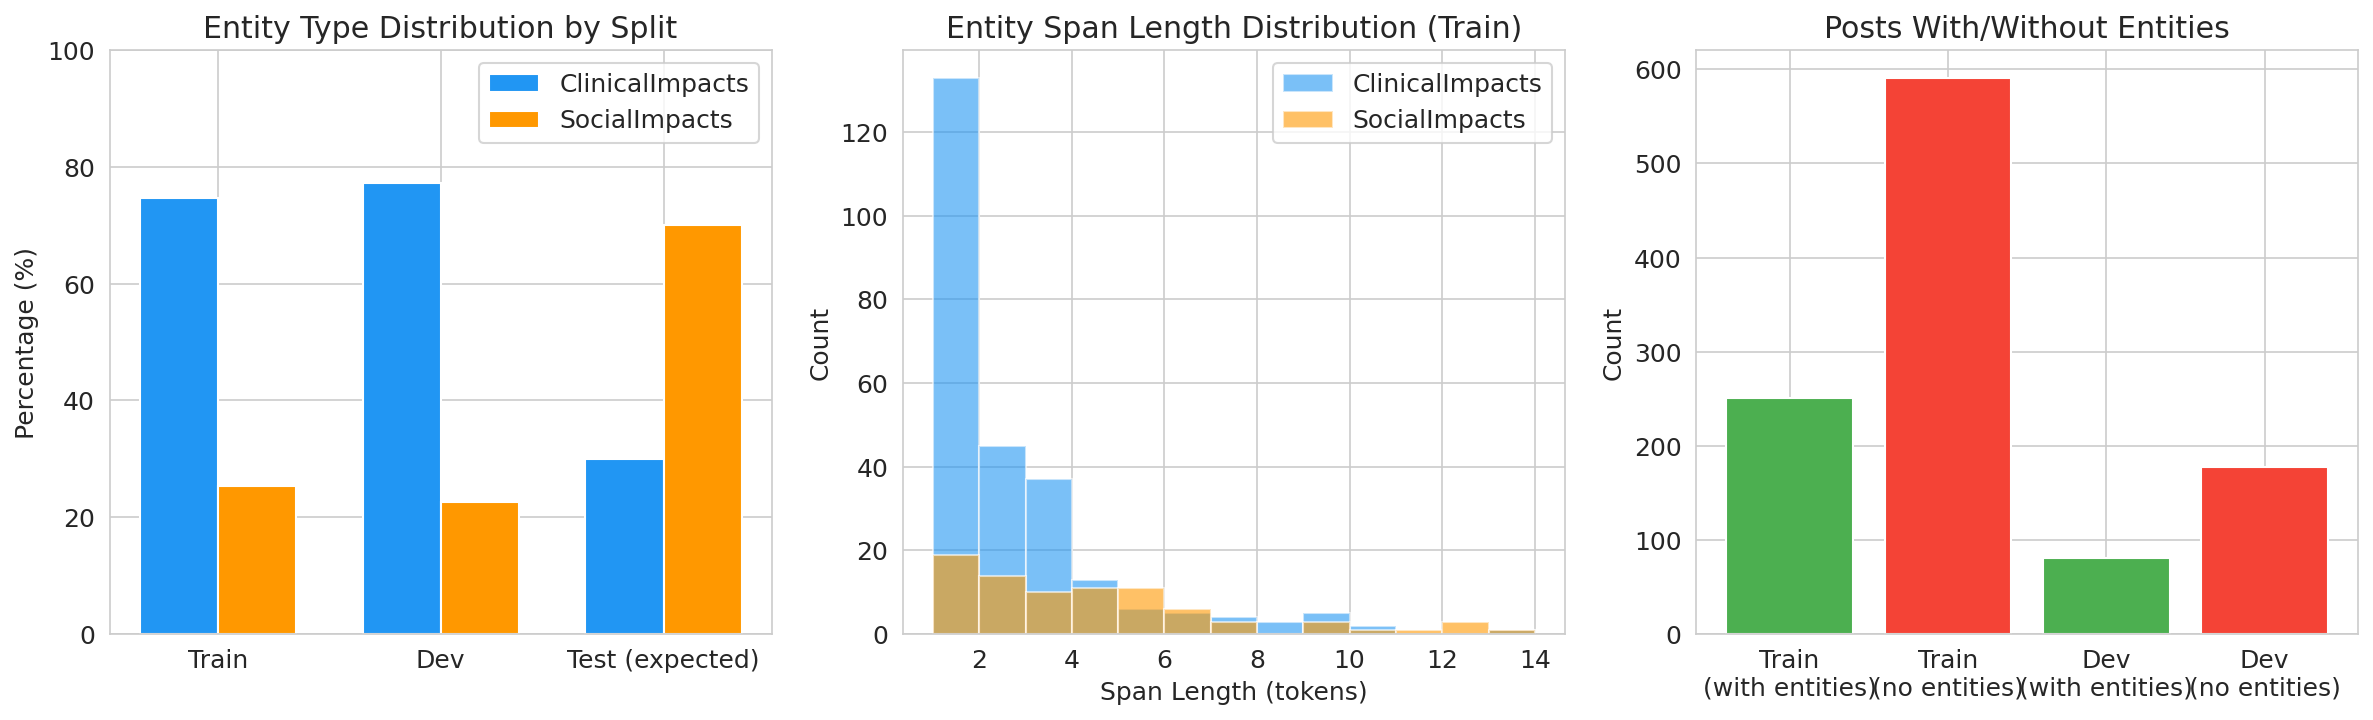
\includegraphics[width=0.92\textwidth]{fig_eda.png}
  \end{center}
  \vspace{-0.8em}
  \scriptsize \textbf{Left:} Train/Dev are Clinical-heavy; Test flips to $\approx$70\,\% Social.
  \textbf{Middle:} Social spans are longer and heavier-tailed than Clinical.
  \textbf{Right:} most Dev posts contain no entities at all.
  \smallskip

  \textbf{Preprocessing as an axis (v2 vs v5).} Every family is run twice -- \textbf{v2}\,$=$ raw text, \textbf{v5}\,$=$ mojibake repair, \texttt{@user}/URL masking, emoji/punctuation scrub, positions restored as \texttt{O} at inference. Both regimes feed the cross-version ensemble search.
\end{frame}

% ---------- 5. Models ----------
\begin{frame}{Model Comparison: Architectures and Backbones}
  \centering
  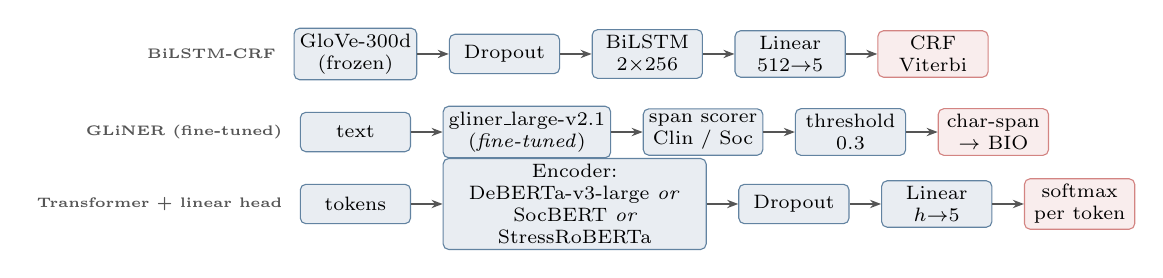
\begin{tikzpicture}[node distance=3mm and 4mm]
    %% --- BiLSTM-CRF ---
    \node[block] (bl_emb) {GloVe-300d\\(frozen)};
    \node[block, right=of bl_emb] (bl_drop) {Dropout};
    \node[block, right=of bl_drop] (bl_lstm) {BiLSTM\\$2{\times}256$};
    \node[block, right=of bl_lstm] (bl_lin) {Linear\\$512{\to}5$};
    \node[op, right=of bl_lin] (bl_crf) {CRF\\Viterbi};
    \draw[arr] (bl_emb) -- (bl_drop);
    \draw[arr] (bl_drop) -- (bl_lstm);
    \draw[arr] (bl_lstm) -- (bl_lin);
    \draw[arr] (bl_lin) -- (bl_crf);
    \node[label, left=1mm of bl_emb] {\textbf{BiLSTM-CRF}};

    %% --- GLiNER fine-tuned ---
    \node[block, below=4mm of bl_emb] (gl_in) {text};
    \node[block, right=of gl_in] (gl_model) {gliner\_large-v2.1\\(\emph{fine-tuned})};
    \node[block, right=of gl_model] (gl_head) {span scorer\\Clin / Soc};
    \node[block, right=of gl_head] (gl_thr) {threshold\\$0.3$};
    \node[op, right=of gl_thr] (gl_bio) {char-span\\$\to$ BIO};
    \draw[arr] (gl_in) -- (gl_model);
    \draw[arr] (gl_model) -- (gl_head);
    \draw[arr] (gl_head) -- (gl_thr);
    \draw[arr] (gl_thr) -- (gl_bio);
    \node[label, left=1mm of gl_in] {\textbf{GLiNER (fine-tuned)}};

    %% --- Transformer token classifier (shared head, different encoders) ---
    \node[block, below=4mm of gl_in] (tc_in) {tokens};
    \node[block, right=of tc_in, text width=3.2cm] (tc_enc) {Encoder:\\DeBERTa-v3-large \emph{or}\\SocBERT \emph{or} StressRoBERTa};
    \node[block, right=of tc_enc] (tc_drop) {Dropout};
    \node[block, right=of tc_drop] (tc_lin) {Linear\\$h{\to}5$};
    \node[op, right=of tc_lin] (tc_sm) {softmax\\per token};
    \draw[arr] (tc_in) -- (tc_enc);
    \draw[arr] (tc_enc) -- (tc_drop);
    \draw[arr] (tc_drop) -- (tc_lin);
    \draw[arr] (tc_lin) -- (tc_sm);
    \node[label, left=1mm of tc_in] {\textbf{Transformer + linear head}};
  \end{tikzpicture}

  \vspace{-1mm}
  \begin{center}\scriptsize
  \begin{tabular}{lc}
    \toprule
    Model & Dev Relaxed F1 (best LR) \\
    \midrule
    BiLSTM-CRF & 0.296 \\
    GLiNER (fine-tuned) & 0.524 \\
    SocBERT (Reddit-domain) & 0.404 \\
    StressRoBERTa (mental-health) & 0.482 \\
    DeBERTa-v3-large baseline & \textbf{0.595} \\
    \bottomrule
  \end{tabular}
  \end{center}
  \scriptsize General-purpose DeBERTa dominates; domain-adapted encoders underperform; zero-shot GLiNER bottoms out at $0.317$ so fine-tuning is essential. Every innovation from here builds on DeBERTa.
\end{frame}

% ---------- 6. Roadmap of Innovations ----------
\begin{frame}{Our Strategy: Seven Contribution Buckets Beyond the Baselines}
  \footnotesize
  \begin{enumerate}\setlength{\itemsep}{0pt}
    \item \textbf{Loss/prompt/multitask ablations} -- focal loss, definition prompting, multi-task head, synthetic-data curriculum.
    \item \textbf{Advanced regularization} -- O-class downweighting (recall-boost), R-Drop, FGM $+$ SWA.
    \item \textbf{Preprocessing as an axis} -- raw (v2) vs cleaned (v5) runtime regimes.
    \item \textbf{Structured prediction pipelines} -- hierarchical DeBERTa, two-step extract$\to$classify, joint sentence$+$token heads, span-nested GLiNER.
    \item \textbf{Domain-adapted backbones} -- SocBERT (Reddit), StressRoBERTa (mental health).
    \item \textbf{Weight-space model soup} -- top-$K$ checkpoint averaging.
    \item \textbf{Prediction-space ensemble search} -- exhaustive subsets, majority vote and probability averaging.
  \end{enumerate}
  \vfill
  \textcolor{neutral}{\footnotesize Each innovation is evaluated with a small LR sweep [2e-5, 5e-5] and the best LR per family is reported.}
\end{frame}

% ---------- 7. Innovation 1: Focal Loss ----------
\begin{frame}{Innovation 1: Distribution-Aware Focal Loss}
  \textbf{Definition.} Let $p_t$ be the predicted probability of the \emph{true} class for a token.
  Standard cross-entropy is $\text{CE}(p_t) = -\log p_t$. Focal loss adds a modulating factor:
  \smallskip

  \begin{center}
  $\displaystyle \mathcal{L}_{\text{focal}}(p_t) \;=\; -\,\alpha_t \, (1 - p_t)^{\gamma}\,\log p_t$
  \end{center}
  \smallskip

  \footnotesize
  \begin{itemize}\setlength{\itemsep}{0pt}
    \item \textbf{$(1 - p_t)^{\gamma}$ -- focusing term.} When the model is already confident ($p_t \to 1$), the factor $\to 0$, so easy tokens contribute almost nothing to the gradient. Hard tokens ($p_t$ small) keep near-full loss. We use $\gamma = 2.0$.
    \item \textbf{$\alpha_t$ -- per-class weight.} Lets us emphasize under-represented classes. We use $\alpha_{\text{Social}} = 1.5$, $\alpha_{\text{Clinical}} = \alpha_{\text{O}} = 1.0$ to push the model toward Social (which dominates the test set).
  \end{itemize}
  \smallskip

  \begin{center}\scriptsize
  \begin{tabular}{lcc}
    \toprule
    & Relaxed F1 & Strict F1 \\
    \midrule
    DeBERTa baseline & \textbf{0.595} & 0.409 \\
    + Focal loss ($\gamma{=}2$, $\alpha_{\text{Soc}}{=}1.5$) & 0.541 & 0.341 \\
    \bottomrule
  \end{tabular}
  \end{center}

  \footnotesize \textbf{Finding:} aggressive Social reweighting pushes the model to \emph{over}-fire on Social tokens ($-0.054$ / $-0.068$). \textcolor{neutral}{Distribution shift is real, but class weighting is the wrong lever for it.}
\end{frame}

% ---------- 8a. Innovation 2 ----------
\begin{frame}{Innovation 2: Definition Prompting}
  Prepend natural-language \emph{definitions} of both entity types before the post; mask them from the loss.
  \medskip

  \begin{center}\scriptsize
  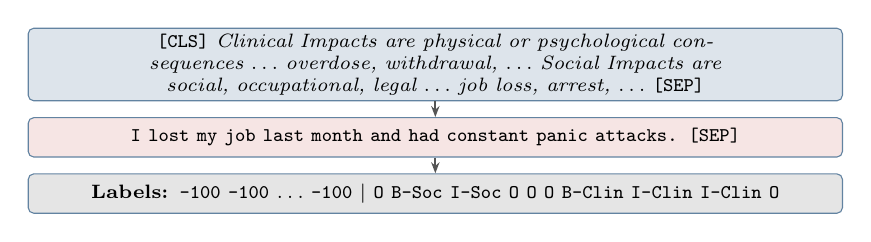
\begin{tikzpicture}[node distance=2mm]
    \node[block, fill=brand!15, text width=10.2cm] (def) {%
      \texttt{[CLS]} \textit{Clinical Impacts are physical or psychological consequences $\ldots$ overdose, withdrawal, $\ldots$ Social Impacts are social, occupational, legal $\ldots$ job loss, arrest, $\ldots$} \texttt{[SEP]}};
    \node[block, fill=accent!15, below=of def, text width=10.2cm] (text) {%
      \texttt{I lost my job last month and had constant panic attacks. [SEP]}};
    \node[block, fill=neutral!15, below=of text, text width=10.2cm] (labels) {%
      \textbf{Labels:} \texttt{-100 -100 $\ldots$ -100} $\mid$ \texttt{O B-Soc I-Soc O O O B-Clin I-Clin I-Clin O}};
    \draw[arr] (def) -- (text);
    \draw[arr] (text) -- (labels);
  \end{tikzpicture}
  \end{center}
  \smallskip

  \footnotesize \textbf{Mechanism:} \texttt{-100} on prefix $\Rightarrow$ definition tokens contribute \emph{attention context} but no gradient. The encoder sees an explicit label ontology on every example.

  \begin{center}\footnotesize
  \begin{tabular}{lcc}
    \toprule
    & Relaxed F1 & Strict F1 \\
    \midrule
    DeBERTa baseline & 0.595 & 0.409 \\
    + Definition prompting & \textbf{0.613} ($+0.018$) & \textbf{0.410} \\
    \bottomrule
  \end{tabular}
  \end{center}
  \vspace{-0.4em}
  \footnotesize \textbf{Best single-model recipe in the project.}
\end{frame}

% ---------- 8b. Innovation 3 ----------
\begin{frame}{Innovation 3: Multi-task Auxiliary Head}
  Share the DeBERTa encoder between token NER and a sentence-level \emph{entity-presence} classifier.

  \begin{center}\scriptsize
  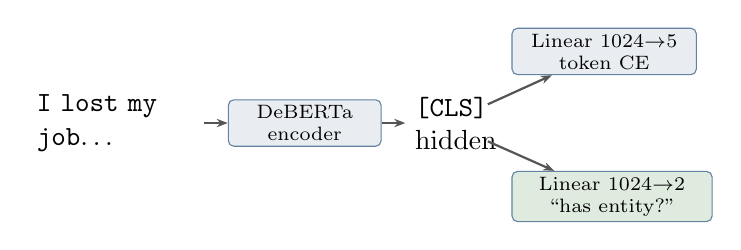
\begin{tikzpicture}[node distance=1.5mm and 3mm]
    \node[text width=2.0cm] (toks) {\texttt{I lost my job$\ldots$}};
    \node[block, right=of toks, text width=1.8cm] (enc) {DeBERTa\\encoder};
    \node[right=of enc, text width=0.8cm] (cls) {\texttt{[CLS]}\\hidden};
    \node[block, above right=of cls, text width=2.2cm] (main) {Linear $1024{\to}5$\\token CE};
    \node[block, below right=of cls, fill=good!15, text width=2.4cm] (aux) {Linear $1024{\to}2$\\``has entity?''};
    \draw[arr] (toks) -- (enc);
    \draw[arr] (enc) -- (cls);
    \draw[arr] (cls) -- (main);
    \draw[arr] (cls) -- (aux);
  \end{tikzpicture}
  \end{center}

  \footnotesize
  % \textbf{Losses.} $\displaystyle \mathcal{L} = \text{CE}_{\text{token}} + 0.3 \cdot \text{CE}_{\text{presence}},$ where
  % $\mathcal{L}_{\text{presence}} = \mathbf{1}[\text{sentence has any B/I tag}]$.
  \textbf{Losses.} $\displaystyle \mathcal{L} = \text{CE}_{\text{token}} + 0.3 \cdot \text{CE}_{\text{presence}},$ where
  the target for $\text{CE}_{\text{presence}}$ is $y = \mathbf{1}[\text{sentence has any B/I tag}]$.
  \smallskip

  \textbf{Result.} Relaxed F1 $= 0.581$ ($-0.014$ vs baseline $0.595$).
  \smallskip

  \textbf{Under the LR sweep, multi-task \emph{slightly hurts} at the token level} -- the auxiliary signal competes with the token objective for encoder capacity on this small dataset. But the multi-task head is a strong feature extractor for later recipes: the recall-boost runs and several ensemble members build on top of it.
\end{frame}

% ---------- 9. Innovation 4: Recall Boost ----------
\begin{frame}{Innovation 4: Recall Boost via O-class Downweighting}
  \textbf{Diagnosis.} Error analysis showed recall lagging precision:
  29 missed spans, 13 of them single-token implicit expressions.
  \medskip

  \textbf{Intervention.} Cross-entropy weight on the \texttt{O} class: $1.0 \to 0.2$.
  Entity classes keep weight $1.0$ while Social classes increases to $1.5$. Combined with multi-task.
  \medskip

  \begin{center}\small
  \begin{tabular}{lcc}
    \toprule
    & Relaxed F1 & Strict F1 \\
    \midrule
    \textbf{DeBERTa baseline} & \textbf{0.595} & \textbf{0.409} \\
    Recall-Boost (seed 42) & 0.582 & 0.312 \\
    Recall-Boost (seed 123) & 0.562 & 0.357 \\
    \bottomrule
  \end{tabular}
  \end{center}
  \medskip

  \textbf{Effect:} the relaxed-F1 gain flips negative under the LR sweep ($-0.013$), and strict F1 drops noticeably -- the O-downweight trades precision for recall.
  Not a blockbuster alone, \emph{but} it produces errors that complement the other recipes --
  which matters for the ensemble.
\end{frame}

% ---------- 11. Innovation 5: R-Drop ----------
\begin{frame}{Innovation 5: R-Drop Consistency Regularization}
  Two stochastic forward passes on the \emph{same} batch, then force their distributions to agree.
  \medskip

  \centering
  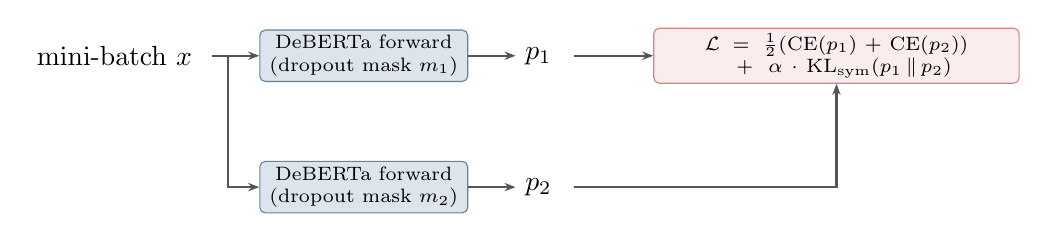
\begin{tikzpicture}[node distance=4mm and 6mm]
    \node[text width=2.1cm] (batch) {mini-batch $x$};
    \node[block, right=of batch, fill=brand!15, text width=2.5cm] (fwd1) {DeBERTa forward\\(dropout mask $m_1$)};
    \node[right=of fwd1, text width=0.5cm] (p1) {$p_1$};
    \node[block, below=10mm of fwd1, fill=brand!15, text width=2.5cm] (fwd2) {DeBERTa forward\\(dropout mask $m_2$)};
    \node[right=of fwd2, text width=0.5cm] (p2) {$p_2$};
    \node[op, right=10mm of p1, text width=4.5cm] (loss) {%
      $\mathcal{L} = \tfrac{1}{2}(\text{CE}(p_1) + \text{CE}(p_2))$\\$\; +\; \alpha\cdot \mathrm{KL}_{\mathrm{sym}}(p_1 \,\|\, p_2)$};
    \draw[arr] (batch) -- (fwd1);
    \draw[arr] (batch.east) -- ++(2mm,0) |- (fwd2.west);
    \draw[arr] (fwd1) -- (p1);
    \draw[arr] (fwd2) -- (p2);
    \draw[arr] (p1) -- (loss);
    \draw[arr] (p2.east) -| (loss.south);
  \end{tikzpicture}
  \medskip

  \footnotesize
  $\alpha = 1.0$, symmetric KL over non-masked tokens only. \\
  No new parameters --
  dropout itself is used as a regularizer that penalizes unstable predictions.
  \medskip

  \begin{center}\footnotesize
  \begin{tabular}{lcc}
    \toprule
    & Relaxed F1 & $\Delta$ vs baseline \\
    \midrule
    DeBERTa baseline & 0.595 & -- \\
    + R-Drop (seed 123) & 0.577 & $-0.018$ \\
    \bottomrule
  \end{tabular}
  \end{center}
\end{frame}

% ---------- 11b. Innovation 6: FGM + SWA ----------
\begin{frame}{Innovation 6: FGM Adversarial + SWA}
  \begin{columns}[T,onlytextwidth]
    \column{0.48\textwidth}
    \textbf{FGM} (per training step)
    \smallskip

    \centering
    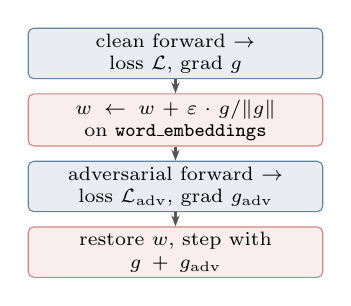
\begin{tikzpicture}[node distance=1.8mm and 3mm]
      \node[block, text width=3.6cm] (f1) {clean forward $\to$\\loss $\mathcal{L}$, grad $g$};
      \node[op, below=of f1, text width=3.6cm] (pert) {$w \leftarrow w + \varepsilon \cdot g / \lVert g \rVert$\\on \texttt{word\_embeddings}};
      \node[block, below=of pert, text width=3.6cm] (f2) {adversarial forward $\to$\\loss $\mathcal{L}_{\text{adv}}$, grad $g_{\text{adv}}$};
      \node[op, below=of f2, text width=3.6cm] (rest) {restore $w$, step with\\$g + g_{\text{adv}}$};
      \draw[arr] (f1) -- (pert);
      \draw[arr] (pert) -- (f2);
      \draw[arr] (f2) -- (rest);
    \end{tikzpicture}
    \smallskip

    \scriptsize $\varepsilon = 0.5$; perturbation lives only on the embedding layer.

    \column{0.48\textwidth}
    \textbf{SWA} (stochastic weight averaging)
    \smallskip

    \centering
    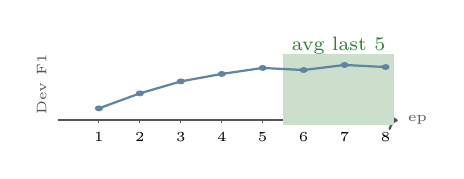
\begin{tikzpicture}[x=0.52cm,y=0.38cm]
      \draw[neutral,->,thick] (0,0) -- (8.3,0) node[right,font=\tiny]{ep};
      \foreach \e in {1,2,...,8}{\draw[neutral,thin] (\e,0) -- (\e,-0.08);\node[font=\tiny, below=0pt] at (\e,-0.08) {\e};}
      \fill[good!25] (5.5,-0.15) rectangle (8.2,2.2);
      \node[font=\scriptsize, good] at (6.85,2.5) {avg last 5};
      \foreach \e/\y in {1/0.4,2/0.9,3/1.3,4/1.55,5/1.75,6/1.68,7/1.85,8/1.78}
        {\fill[brand!70] (\e,\y) circle (0.1);}
      \draw[brand!70,thick]
        (1,0.4) -- (2,0.9) -- (3,1.3) -- (4,1.55) -- (5,1.75) -- (6,1.68) -- (7,1.85) -- (8,1.78);
      \node[font=\tiny, neutral, rotate=90] at (-0.4,1.2) {Dev F1};
    \end{tikzpicture}
    \smallskip

    \scriptsize After epoch 10, running mean of \texttt{state\_dict} over remaining epochs $\to$ final checkpoint. Smooths end-of-training oscillation.
  \end{columns}
  \vfill

  \begin{center}\footnotesize
  \begin{tabular}{lcc}
    \toprule
    & Relaxed F1 & $\Delta$ vs baseline \\
    \midrule
    DeBERTa baseline & 0.595 & -- \\
    + FGM + SWA (seed 42) & 0.573 & $-0.022$ \\
    \bottomrule
  \end{tabular}
  \end{center}
  \vspace{-0.3em}
  \footnotesize Robustness recipe: modestly below the raw baseline on dev, but produces diverse errors the ensemble leverages.
\end{frame}

% ---------- 11b. Training dynamics ----------
\begin{frame}{Training Dynamics Across Recipes}
  \vspace{-0.8em}
  \begin{center}
    
\includegraphics[width=0.64\textwidth]{fig_training_curves.png}
  \end{center}
  \vspace{-1.0em}
  \scriptsize
  \textbf{Top row:} Definition Prompting (orange) tops both Relaxed and Strict F1 from
  epoch~4 onward -- the clearest single-recipe win.
  \textbf{Bottom row:} Dev loss separates recipes even when F1 curves look close; Sentence+Token
  Hierarchy drifts up after epoch~6, signalling mild overfit.
\end{frame}

% ---------- 11c. Structured prediction pipelines ----------
\begin{frame}{Structured Prediction Pipelines}
  \footnotesize
  Four structured variants on top of DeBERTa, each testing a different inductive bias:
  \vspace{-0.3em}
  \begin{center}\scriptsize
  \begin{tabular}{p{3.9cm}p{6.7cm}c}
    \toprule
    Pipeline & Idea & Relaxed F1 \\
    \midrule
    \textbf{Hierarchical DeBERTa} & \texttt{[CLS]} sentence classifier gates a multi-task NER; 10\,\% of no-impact rows kept & \textbf{0.604} \\[2pt]
    Two-Step Impact Pipeline & Stage 1: binary span extraction; Stage 2: clinical / social classifier per span & 0.534 \\[2pt]
    Sentence $+$ Token Hierarchy & One model with joint sentence presence head and token BIO head & 0.530 \\[2pt]
    Span-nested GLiNER & Span scorer with nested-span enumeration and overlap-aware decoding & 0.443 \\
    \bottomrule
  \end{tabular}
  \end{center}
  \vspace{-0.3em}
  \textbf{Hierarchical DeBERTa} is the clear winner and anchors the winning ensemble on the next slide.
  The two-step and joint-hierarchy variants are close to each other but noticeably below the plain token classifier baseline ($0.595$); span-nested GLiNER plateaus much lower.
  \medskip

  \textcolor{neutral}{\scriptsize \textbf{Model soup (weight-space aggregation).} Orthogonal to everything above: average top-$K$ dev-F1 checkpoints from a single LR sweep ($\bar\theta = \tfrac{1}{K}\sum_k \theta_k$). Best soup: recall-boost s42 top-3 at $0.595$ (strict $+0.033$). Soup is only defined for same-architecture runs -- GLiNER, BiLSTM, and every pipeline family above are \emph{not} soupable.}
\end{frame}

% ---------- 12. Ensemble ----------
\begin{frame}{Innovation 7: Ensemble Search -- Majority Vote Beats SOTA}
  \scriptsize
  \textbf{Two complementary searches}, both exhaustive over size-2--5 subsets:
  \begin{itemize}\setlength{\itemsep}{0pt}
    \item \textbf{Majority vote, cross-version:} top-7 relaxed $+$ top-7 strict from each regime (v2 / v5) $\Rightarrow$ 28 candidates, \textbf{122{,}409 combinations}. Operates on BIO tag sequences -- every family is eligible.
    \item \textbf{Probability average, v2-only:} 7 candidates, 112 combinations. Averages per-token class distributions, so GLiNER span models and structured pipelines are excluded.
  \end{itemize}

  \begin{center}\scriptsize
  \begin{tabular}{lcccc}
    \toprule
    Ensemble & Relaxed F1 & Strict F1 & Precision & Recall \\
    \midrule
    2 models (majority) & 0.623 & 0.465 & 0.586 & 0.664 \\
    3 models (majority) & 0.621 & 0.507 & 0.638 & 0.605 \\
    \rowcolor{good!15}
    \textbf{4 models (majority)} & \ours & 0.509 & 0.648 & 0.623 \\
    5 models (majority) & 0.631 & \textbf{0.518} & 0.670 & 0.597 \\
    \midrule
    Best probability average (v2, 7 cand.) & 0.614 & 0.431 & 0.653 & 0.580 \\
    \bottomrule
  \end{tabular}
  \end{center}
  \medskip

  \textbf{Best ensemble:} hierarchical-pipeline anchor $+$ 3 complementary DeBERTa recipes across both regimes. \textbf{Beats published SOTA \sota{} on dev} ($+0.025$). Hard voting $>$ soft averaging here ($0.635$ vs $0.614$).
\end{frame}

% ---------- 13. Full Ablation ----------
\begin{frame}{Full Ablation Table (LR-Selected per Family)}
  \centering\tiny
  \begin{tabular}{lcccc}
    \toprule
    Model & Relaxed F1 & Strict F1 & Best LR & Epoch \\
    \midrule
    BiLSTM-CRF & 0.296 & 0.256 & 5e-4 & 15 \\
    GLiNER (fine-tuned) & 0.524 & -- & 2e-5 & -- \\
    \quad Span-nested GLiNER & 0.443 & -- & 1e-5 & -- \\
    SocBERT baseline & 0.404 & 0.277 & 5e-5 & -- \\
    StressRoBERTa baseline & 0.482 & 0.270 & 2e-5 & -- \\
    DeBERTa baseline & 0.595 & 0.409 & 2e-5 & 7 \\
    \quad + Focal loss & 0.541 & 0.341 & 2e-5 & 6 \\
    \quad + Multi-task & 0.581 & 0.382 & 5e-5 & 9 \\
    \textbf{\quad + Definition prompting} & \bestsingle & \textbf{0.410} & 5e-5 & 5 \\
    Hierarchical DeBERTa pipeline & 0.604 & 0.372 & 2e-5 & -- \\
    Two-Step Impact Pipeline & 0.534 & 0.404 & 2e-5 & -- \\
    Sentence + Token Hierarchy & 0.530 & 0.374 & 5e-5 & -- \\
    Recall-Boost (seed 42) & 0.582 & 0.312 & 2e-5 & 7 \\
    R-Drop (seed 123) & 0.577 & 0.380 & 2e-5 & 9 \\
    FGM + SWA (seed 42) & 0.573 & 0.356 & 2e-5 & 10 \\
    Model soup (recall-boost s42) & 0.595 & 0.331 & 2e-5 & -- \\
    \rowcolor{good!15}
    \textbf{4-Model Ensemble (majority vote)} & \ours & \textbf{0.509} & -- & -- \\
    \midrule
    \textit{GPT-4o 3-shot (reported)} & \textit{0.440} & -- & -- & -- \\
    \textit{DeBERTa (published SOTA)} & \textit{0.610} & -- & -- & -- \\
    \bottomrule
  \end{tabular}
  \vfill
  \footnotesize Dev-set evaluation. Each family has its own LR sweep; the row reports the best LR.
\end{frame}

% ---------- 14. Error Analysis ----------
\begin{frame}{Error Analysis on the Best Single Model}
  Definition Prompting (lr\,5e-5), Relaxed F1 $= 0.613$, Strict F1 $= 0.410$.
  \medskip
  \begin{columns}[T,onlytextwidth]
    \column{0.48\textwidth}
      \textbf{Error categories (Dev)}
      \begin{itemize}
        \item \textbf{Boundary errors} dominate -- Relaxed/Strict gap of $\approx 0.20$.
        \item Missed spans concentrated on single-token implicit expressions.
        \item Long multi-word Social spans get partial matches.
        \item Type confusion is rare.
      \end{itemize}
    \column{0.48\textwidth}
      \textbf{Qualitative observations}
      \begin{itemize}
        \item Implicit: ``those weeks were hell'' often missed.
        \item ``charged with disorderly conduct'' $\to$ partial span.
        \item Negated phrases correctly rejected.
        \item Third-person references are mostly ignored.
      \end{itemize}
  \end{columns}
  \vfill
  \textcolor{neutral}{\footnotesize Boundary errors and implicit false negatives are the two buckets that would pay off most for future work.}
\end{frame}

% ---------- 15. Key Insights ----------
\begin{frame}{Three Key Insights}
  \begin{enumerate}
    \item \textbf{LR sweeps are non-negotiable.}
          Best LR is family-specific (2e-5 for baseline, 5e-5 for definition prompting and multi-task);
          a single global LR masks the true ordering between recipes and flips several conclusions.
    \smallskip
    \item \textbf{Training-objective diversity beats individual model polish.}
          Single models plateau around $0.60$; a 4-model majority-vote ensemble
          climbs to \ours{} -- a $+0.04$ jump from combining \emph{different recipes}
          (hierarchical, definition, recall-boost, R-Drop), not more seeds of the same one.
    \smallskip
    \item \textbf{Majority vote beats probability averaging.}
          On this small, noisy dev set, hard voting ($0.635$) is more robust
          than soft averaging ($0.614$). Confident-but-occasionally-wrong
          models don't combine well via logits.
  \end{enumerate}
\end{frame}

% ---------- 16. Limitations ----------
\begin{frame}{Limitations \& Future Work}
  \textbf{Limitations}
  \begin{itemize}
    \item Dev-set only -- no test-set access; numbers will likely shift under the real 70\,\% Social distribution.
    \item Our ensemble beats the published SOTA ($0.635$ vs $0.610$) on dev, but 258 samples is a noisy reference -- the gap needs test-set confirmation.
    \item Single-sentence inputs -- no cross-post user-history context.
  \end{itemize}
  \medskip

  \textbf{Future work}
  \begin{itemize}
    \item LLM-synthesized data (Claude / GPT-4o) targeting implicit Social cases.
    \item Greedy forward selection for principled ensemble membership.
    \item Cross-domain transfer from biomedical NER corpora.
    \item Instruction-tuned Llama-3 with task-specific prompts.
  \end{itemize}
\end{frame}

% ---------- 17. Summary ----------
\begin{frame}{Summary}
  \begin{itemize}
    \item \textbf{Task:} BIO NER for Clinical/Social impacts of substance use on Reddit.
    \item \textbf{Models:} BiLSTM-CRF, GLiNER (fine-tuned), SocBERT, StressRoBERTa, DeBERTa-v3-large.
    \item \textbf{7 contribution buckets:} ablations, advanced regularization, preprocessing axis, structured pipelines, domain backbones, model soup, ensemble search -- each evaluated under an LR sweep.
    \item \textbf{Best single model:} Definition Prompting, $F_{1} = \bestsingle$ (exceeds baseline by $+0.018$).
    \item \textbf{Best system:} 4-model majority-vote ensemble,
          $F_{1} = \ours$, clearly beating the published SOTA \sota{} on dev ($+0.025$).
    \item \textbf{Main takeaway:} training-objective diversity + majority voting $>$ any single-model trick we tried.
  \end{itemize}
\end{frame}

% % ---------- 18. Thanks ----------
% \begin{frame}[standout]
%   Thank you.\\
%   \vspace{1em}
%   \Large Questions?
% \end{frame}

\end{document}
